% xetex compatible variant that support TTF fonts according to company rules
\documentclass[ignorenonframetext, professionalfonts, hyperref={unicode}]{beamer}

\usetheme{Epam}

\usepackage{fontspec}
\setsansfont{SourceSansPro-Regular}
%\setbeamerfont{frametitle}{family=\fontspec{Oswald}}
\setbeamerfont{frametitle}{family=\fontspec{Oswald}}
\setbeamerfont{block title}{family=\fontspec{Oswald}}

%\setmainfont{Times New Roman}
\defaultfontfeatures{Mapping=tex-text}
\defaultfontfeatures{Ligatures=TeX}

%\setsansfont{Arial}
%\setromanfont{Trebuchet MS}

\usepackage{cmap}
\usepackage{graphicx}

\usepackage{textcomp}

\usepackage{beamerthemesplit}

\usepackage{ulem}

\usepackage{verbatim}
\usepackage{import}

\usepackage{listings}
\lstloadlanguages{bash}

\lstset{escapechar=`,
	captionpos=b,
	extendedchars=false,
	language=sh,
%	frame=single,
	tabsize=2, 
	columns=fullflexible, 
%	basicstyle=\scriptsize,
	keywordstyle=\color{blue}, 
	commentstyle=\itshape\color{brown},
%	identifierstyle=\ttfamily, 
	stringstyle=\mdseries\color{green}, 
	showstringspaces=false, 
	numbers=left, 
	numberstyle=\footnotesize, 
	breaklines=true, 
	inputencoding=utf8,
	keepspaces=true,
	morekeywords={u\_short, u\_char, u\_long, in\_addr}
	}

\definecolor{darkgreen}{cmyk}{0.7, 0, 1, 0.5}

\lstdefinelanguage{diff}
{
    morekeywords={+, -},
    sensitive=false,
    morecomment=[l]{//},
    morecomment=[s]{/*}{*/},
    morecomment=[l][\color{darkgreen}]{+},
    morecomment=[l][\color{red}]{-},
    morestring=[b]",
}

\author[Epam]{{\bf Epam}\\Low Level Programming Department}

%\institution[EPAM]{EPAM}
%\logo{\includegraphics[width=1cm]{logo.png}}

\graphicspath{{../../slides/cmdline/clipart/}{../../slides/bash/clipart/}}

\bibliographystyle{unsrt}
\setbeamertemplate{bibliography item}{\insertbiblabel}

\AtBeginSection[]{%
  \begin{frame}<beamer>
    \frametitle{}
    \tableofcontents[
        sectionstyle=show/shaded, hideallsubsections ]
  \end{frame}
  \addtocounter{framenumber}{-1}% If you don't want them to affect the slide number
}

% \regex for regular expressions
\newcommand{\regex}[1]{ %
\expandafter{$\ulcorner{\color{blue}\texttt{#1}}\lrcorner$} %
}



\title{Введение в GNU/Linux}


%%%%%%%%%%%%%%%%%%%%%%%%%%%%%%%%%%%%%%%%%%%%%%%%%
%%%%%%%%%% Begin Document  %%%%%%%%%%%%%%%%%%%%%%
%%%%%%%%%%%%%%%%%%%%%%%%%%%%%%%%%%%%%%%%%%%%%%%%%

\begin{document}

\begin{frame}
	\frametitle{}
	\titlepage
	\vspace{-0.5cm}
	\begin{center}
	%\frontpagelogo
	\end{center}
\end{frame}


%%%%%%%%%%%%%%%%%%%%%%%%%%%%%%%%%%%%%%%%%   
%%%%%%%%%% Content starts here %%%%%%%%%%
%%%%%%%%%%%%%%%%%%%%%%%%%%%%%%%%%%%%%%%%%

\section{File permissions}
\subsection{Umask}
\mode<all>{\begin{frame}[fragile]{Special modes}

\begin{block}{SUID (set user ID), SGID (set group ID) }
Установка битов SUID или SGID позволит пользователям запускать исполняемые файлы от имени владельца (или группы) запускаемого файла
\end{block}
\verb|chmod 4755 plu.txt| или \verb|chmod u+s plu.txt|

\begin{block}{Sticky bit mode}
Каталог с установленным sticky-битом означает, что удалить файл из этого каталога может только владелец файла 
\end{block}
\verb|chmod 1755 plu| или \verb|chmod +t plu|

\end{frame}
}
\subsection{SUID bit}
\mode<all>{\begin{frame}[fragile]{Default access mode: umask}

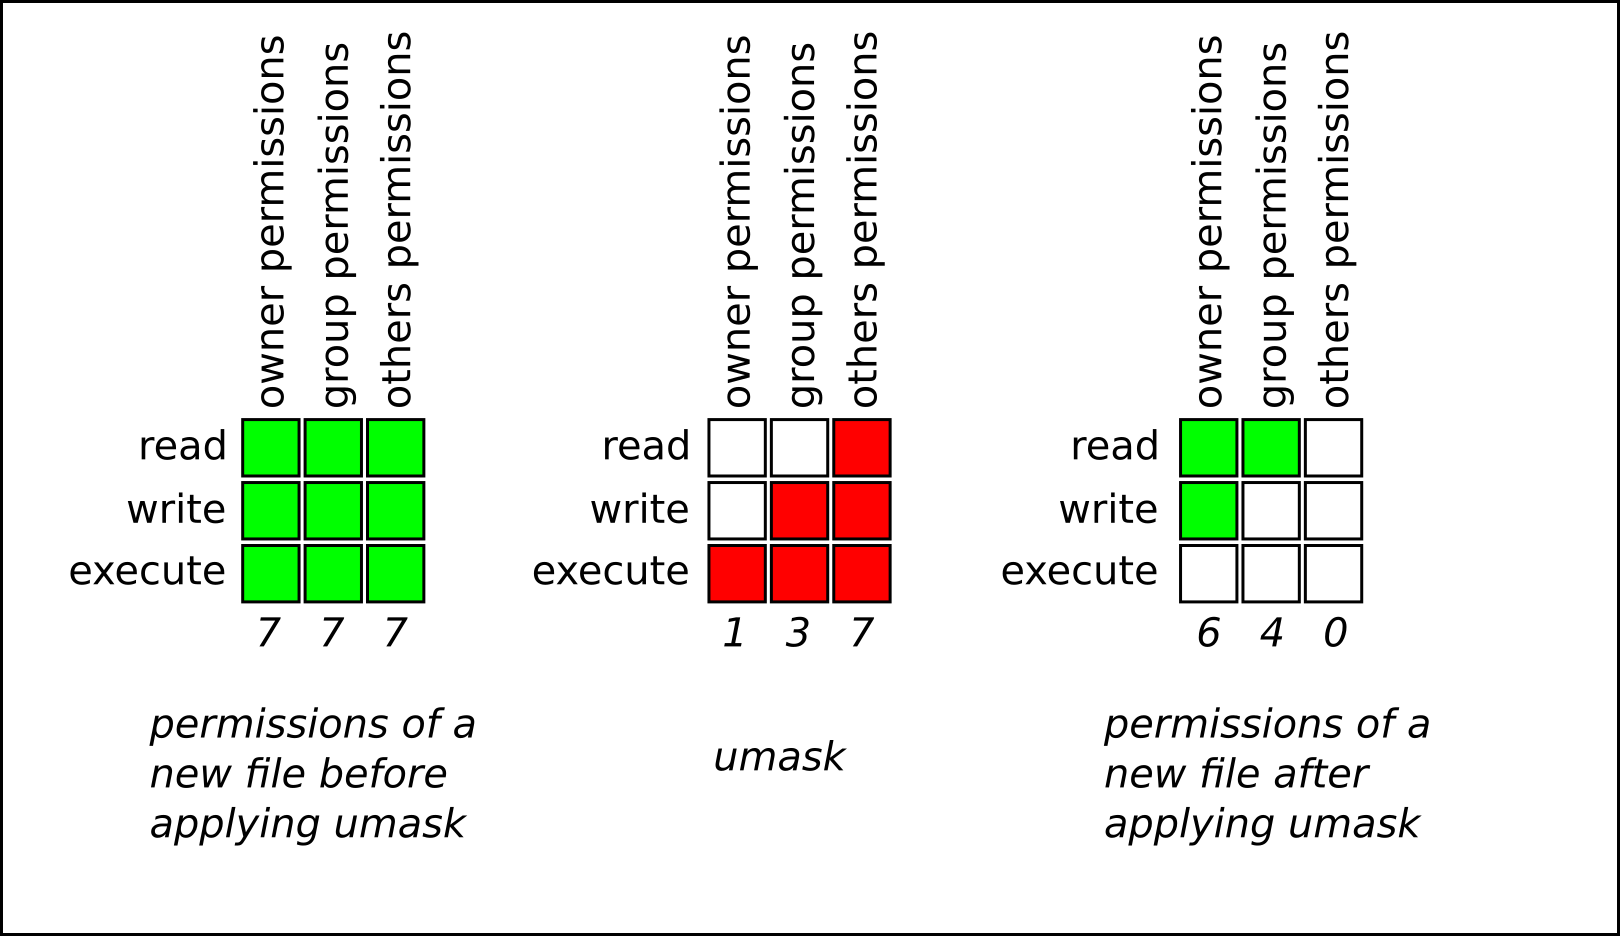
\includegraphics[width=0.9\textwidth]{../../slides/cmdline/clipart/Users_Groups-Umask_Example.png}

\end{frame}
}
\section{OS initialization system.}
\mode<all>{\begin{frame}{init}
	Менеджер управления работой системой и сервисами.
	
	\bigskip

	\center{\large PID = 1}

	\bigskip

	\begin{block}{Наиболее известные}
		\begin{itemize}
			\item SysVInit
			\item systemd
			\item upstart
		\end{itemize}
	\end{block}
\end{frame}

\begin{frame}{SysVInit}
	\begin{block}{Управление}
		\begin{itemize}
			\item kernel boot parameters: <N> -- runlevel
			\item утилита {\tt runlevel}
			\item утилита {\tt init}
		\end{itemize}
	\end{block}

	\scriptsize
	\begin{block}{Runlevel}
		\begin{table}
			\begin{tabular}{| c | l | }
			\hline
			Runlevel & Описание\\
			\hline
			0	& Выключить систему \\
			1,s,single & Однопользовательский режим \\
			2	& Многопользовательский режим без графики. Без сетевых сервисов.\\
			3	& Многопользовательский режим без графики. Полноценная сеть. \\
			4	& Определяется на хосте\\
			5	& Многопользовательский режим с графикой.\\
			6	& Перезагрузка\\
			emergency & Аварийная оболочка \\
			\hline
			\end{tabular}
		\end{table}
	\end{block}
\end{frame}

\begin{frame}{SysVInit: сервисы}
	\begin{block}{Управление}
		\begin{itemize}
			\item утилита {\tt service}
			\item утилита {\tt chkconfig}
		\end{itemize}
	\end{block}

	\begin{block}{Сервисы}
		\begin{itemize}
			\item {\tt /etc/rc.d/init.d}
			\item {\tt /etc/rc.d/rc.N}\footnote{N=runlevel}
		\end{itemize}
	\end{block}
\end{frame}

\begin{frame}{systemd}
	\begin{block}{Управление}
		\begin{itemize}
			\item kernel boot parameters\\
				{\tt systemd.unit=rescue.target} \\
			\item утилита {\tt systemctl} \\
				{\tt systemctl isolate multi-user.target} \\
				{\tt systemctl set-default single.target}
		\end{itemize}
	\end{block}

	\begin{block}{targets}
		\tiny
		\begin{table}
			\begin{tabular}{| c | l | l | }
			\hline
			Runlevel & Описание\\
			\hline
			0	& poweroff.target & Выключить систему \\
			1,s,single & rescue.target  & Однопользовательский режим \\
			2	& multi-user.target & Многопользовательский режим без графики. Без сетевых сервисов.\\
			3	& multi-user.target & Многопользовательский режим без графики. Полноценная сеть. \\
			4	& multi-user.target & Определяется на хосте\\
			5	& graphical.target & Многопользовательский режим с графикой.\\
			6	& reboot.target & Перезагрузка\\
			emergency & emergency.target & Аварийная оболочка \\
			\hline
			\end{tabular}
		\end{table}
	\end{block}
\end{frame}

\begin{frame}{systemd: сервисы}
	\begin{block}{Управление}
		\begin{itemize}
			\item утилита {\tt systemctl}
		\end{itemize}
	\end{block}

	\begin{block}{Сервисы}
		\begin{itemize}
			\item {\tt /lib/systemd/system/}
			\item {\tt /etc/systemd/system/}
		\end{itemize}
	\end{block}
\end{frame}
}

%\section{User management}
%\mode<all>{\input{../../slides/multiuser/account_files.tex}}
%\mode<all>{\input{../../slides/multiuser/pam.tex}}

\section{Configure network settings}
\mode<all>{\begin{frame}{Configure network interface}
Minimal settings are:
  \begin{itemize}
    \item IP address 
    \item Netmask 
	\item Gateway
    \item DNS server (optional)
  \end{itemize}
Why do you need static configuration? \\ 
Dynamic host configuration protocol (DHCP). DHCP server can be built-in:
  \begin{itemize}
	\item Server
    \item Modem 
    \item Hypervisor 
  \end{itemize}
	or run DHCP as standalone service
\end{frame}

\begin{frame}{Network configuration via commands}
\lstinputlisting[language=bash]{../../slides/networking/samples/example_network_configuration.txt}
\end{frame}

\begin{frame}[fragile]{Ubuntu network configuration files}

Configuration file: {\tt /etc/network/interfaces }

\begin{block}{Dynamic IP Address Assignment}
    \begin{lstlisting}
auto eth0
iface eth0 inet dhcp
    \end{lstlisting}
\end{block}

\begin{block}{Static IP Address Assignment}
    \begin{lstlisting}
    auto eth0
    iface eth0 inet static
    address 10.0.0.100
    netmask 255.255.255.0
    gateway 10.0.0.1
    \end{lstlisting}
\end{block}
\end{frame}

\begin{frame}{Network configuration files}
  \begin{itemize}
    \item {\tt /etc/sysconfig/network}
    \item Расположение зависит от дистрибутива:
        \begin{itemize}
            \item RH-like: {\tt /etc/sysconfig/network-scripts}\\
                {\tt /etc/sysconfig/network-scripts/ifcfg-eth0}
            \item ALTLinux: {\tt /etc/net/ifaces}
            \item Debian: {\tt /etc/network/interfaces}
            \item Gentoo: {\tt /etc/conf.d/net}
        \end{itemize}
  \end{itemize}
\end{frame}

\begin{frame}[fragile]{CentOS network configuration files}
Configuration file: {\tt /etc/sysconfig/network-scripts/ifcfg-<interface-name> }

\begin{block}{Dynamic IP Address Assignment}
    \begin{lstlisting}
DEVICE=eth0
BOOTPROTO=dhcp
ONBOOT=yes
    \end{lstlisting}
\end{block}

\begin{block}{Static IP Address Assignment}
    \begin{lstlisting}
DEVICE=eth0
BOOTPROTO=static
ONBOOT=yes
NETMASK=255.255.255.0
IPADDR=10.0.1.27
    \end{lstlisting}
\end{block}
\end{frame}

\begin{frame}[fragile]{Apply configuration settings}
    \begin{lstlisting}
    ifdown eth0
    ifup eth0
    \end{lstlisting}
    CentOS manage network configuration
    \begin{lstlisting}
    systemctl status network.service
    systemctl restart network.service
    \end{lstlisting}
    Ubuntu manage network configuration
    \begin{lstlisting}
    systemctl status networking.service
    systemctl restart networking.service
    \end{lstlisting}
\end{frame}


\begin{frame}[fragile]{Host name resolution}
\begin{block}{ {\tt /etc/resolv.conf}}
        \begin{lstlisting}
        domain it-academy.by
        search it-academy.by
        nameserver 217.23.115.244
        nameserver 192.168.37.1
        \end{lstlisting}
    \end{block}
\begin{block}{ {\tt /etc/hosts} }
        \begin{lstlisting}
        127.0.0.1 localhost
        127.0.1.1 zabbix
        \end{lstlisting}
\end{block}
\end{frame}
}
%\mode<all>{\input{../../slides/networking/interface-management}}

\end{document}
